%% LyX 2.3.6.1 created this file.  For more info, see http://www.lyx.org/.
%% Do not edit unless you really know what you are doing.
\documentclass[english,xcolor=svgnames, handout]{beamer}
\usepackage{amstext}
\usepackage{fontspec}
\setcounter{secnumdepth}{3}
\setcounter{tocdepth}{3}
\usepackage{calc}
\usepackage{graphicx}
\PassOptionsToPackage{normalem}{ulem}
\usepackage{ulem}
\ifx\hypersetup\undefined
  \AtBeginDocument{%
    \hypersetup{unicode=true}
  }
\else
  \hypersetup{unicode=true}
\fi

\makeatletter

%%%%%%%%%%%%%%%%%%%%%%%%%%%%%% LyX specific LaTeX commands.
%% Because html converters don't know tabularnewline
\providecommand{\tabularnewline}{\\}

%%%%%%%%%%%%%%%%%%%%%%%%%%%%%% Textclass specific LaTeX commands.
% this default might be overridden by plain title style
\newcommand\makebeamertitle{\frame{\maketitle}}%
% (ERT) argument for the TOC
\AtBeginDocument{%
  \let\origtableofcontents=\tableofcontents
  \def\tableofcontents{\@ifnextchar[{\origtableofcontents}{\gobbletableofcontents}}
  \def\gobbletableofcontents#1{\origtableofcontents}
}

%%%%%%%%%%%%%%%%%%%%%%%%%%%%%% User specified LaTeX commands.

% you can play with different themes and color themes to find your favorite combination.
\mode<presentation> {
  \usetheme{Luebeck}
  \usecolortheme{beaver}
  \beamertemplatenavigationsymbolsempty
}


\usepackage{graphicx} % for including images
\usepackage{pgf} % for logo
\usepackage{colortbl}
\usepackage{emoji}

\date{} % Date, can be changed to a custom date


\definecolor{blue}{RGB}{38, 122, 181}
\definecolor{orange}{RGB}{255, 128, 0}
\definecolor{lorange}{RGB}{255, 178, 102}
\definecolor{llorange}{RGB}{255, 229,204 }
\definecolor{verylightgray}{RGB}{246, 246, 246}


\setbeamertemplate{itemize item}{\color{orange}$\blacksquare$}
\setbeamertemplate{itemize subitem}{\color{orange}$\blacktriangleright$}

\usepackage{tcolorbox}

\newcommand\blfootnote[1]{%
  \begingroup
  \renewcommand\thefootnote{}\footnote{#1}%
  \addtocounter{footnote}{-1}%
  \endgroup
}

\makeatother

\usepackage{polyglossia}
\setdefaultlanguage[variant=american]{english}
\begin{document}
\title[\textcolor{gray}{ST1101 \hspace{4.45cm}\insertframenumber/\inserttotalframenumber}]{\textcolor{orange}{Statistik och Dataanalys I}}
\subtitle{\textcolor{orange}{Föreläsning 12 - Betingade sannolikheter och Bayes
sats}}
\author[\textbf{\textcolor{gray}{Statistik och Dataanalys I}}]{\textbf{Oskar Gustafsson} \\
\vspace{0.2cm}
\vspace{-0.3cm}
}
\institute[Stockholms universitet]{Statistiska institutionen\\
Stockholms universitet}

\makebeamertitle

\begin{frame}{\textbf{\textcolor{orange}{Översikt}}}
\begin{itemize}
\item \textbf{\textcolor{blue}{Betingad sannolikhet}}
\end{itemize}
\bigskip{}

\begin{itemize}
\item \textbf{\textcolor{blue}{Lagen om total sannolikhet}}\bigskip{}
\item \textbf{\textcolor{blue}{Bayes sats}}
\end{itemize}
\end{frame}

\begin{frame}{\textbf{\textcolor{orange}{Betingad sannolikhet}}}
\begin{itemize}
\item Covid:\medskip{}

\begin{itemize}
\item A = \{positivt hemtest\}, B = \{har covid\}.\medskip{}
\item Intresse: $P(B\vert A)=P(\text{har covid}\vert\text{positivt hemtest})$\medskip{}
\end{itemize}
\item Tecknet \textbf{\textcolor{orange}{|}} läses 'givet' eller betingat
på. \medskip{}
\item Sannolikheten för att $B$ inträffar \textbf{\textcolor{orange}{givet
att A har inträffat}}.\bigskip{}
\end{itemize}
\begin{center}
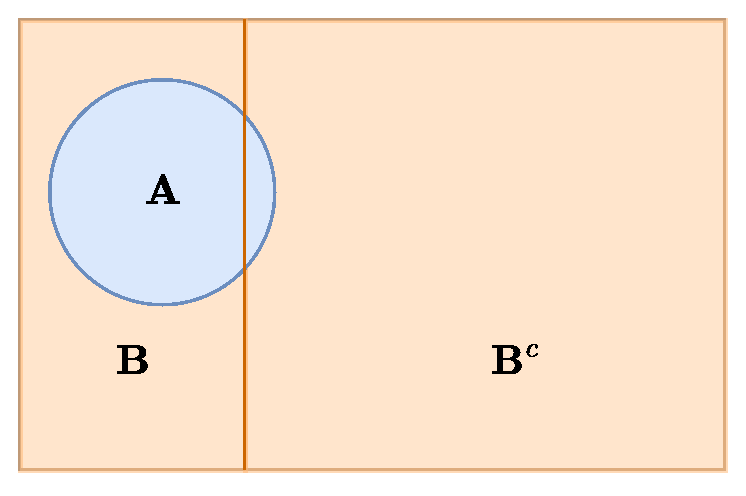
\includegraphics[scale=0.35]{figs/bayes_twoevents}
\par\end{center}

\end{frame}

\begin{frame}{\textbf{\textcolor{orange}{Betingad sannolikhet - världen krymper}}}
\begin{itemize}
\item \textbf{\textcolor{blue}{Betingad sannolikhet}}
\[
P(B|A)=\frac{P(A\cap B)}{P(A)}
\]
\item \textbf{\textcolor{blue}{Betinga på $A$}} innebär att blå cirkeln
blir \textbf{\textcolor{blue}{vårt nya utfallsrum}}. 
\item Inget utanför blå cirkeln kan längre inträffa. “$A$ is the new
$S$”.
\end{itemize}
\begin{center}
\includegraphics[scale=0.35]{figs/conditional_prob_lifting_out}
\par\end{center}

\end{frame}

\begin{frame}{\textbf{\textcolor{orange}{Korstabeller och sannolikheter}}}
\begin{center}
\noindent\begin{minipage}[t]{1\columnwidth}%
\textrm{ }%
\begin{tabular}{c}
Antal\tabularnewline
\includegraphics[scale=0.35]{figs/PetsCounts}\tabularnewline
\end{tabular}\textrm{}%
\begin{tabular}{c}
Snittsannolikheter (Table \%)\tabularnewline
\includegraphics[scale=0.35]{figs/PetsPropTable}\tabularnewline
\end{tabular}%
\end{minipage}
\par\end{center}

\begin{center}
\noindent\begin{minipage}[t]{1\columnwidth}%
\textrm{ }%
\begin{tabular}{c}
Betingat på kön (Column \%)\tabularnewline
\includegraphics[scale=0.34]{figs/PetsPropCols}\tabularnewline
\end{tabular}\textrm{}%
\begin{tabular}{c}
Betingat på husdjur (Row \%)\tabularnewline
\includegraphics[scale=0.35]{figs/PetsPropRows}\tabularnewline
\end{tabular}%
\end{minipage}
\par\end{center}

\end{frame}

\begin{frame}{\textbf{\textcolor{orange}{Korstabell och mosaic-plot}}}
\begin{center}
\includegraphics[scale=0.4]{figs/PetsPropTable}
\par\end{center}

\begin{center}
\includegraphics[scale=0.42]{figs/pets_only_joint}
\par\end{center}

\end{frame}

\begin{frame}{\textbf{\textcolor{orange}{Venndiagram}}}
\begin{center}
\includegraphics[scale=0.75]{figs/venn_cat_dogs}
\par\end{center}

\end{frame}

\begin{frame}{\textbf{\textcolor{orange}{Korstabell och betingad sannolikhet}}}
\begin{center}
\includegraphics[scale=0.5]{figs/PetsPropCols}
\par\end{center}

\end{frame}

\begin{frame}{\textbf{\textcolor{orange}{Korstabell och betingad sannolikhet}}}
\begin{center}
\includegraphics[scale=0.42]{figs/pets_mosaic_conditional}
\par\end{center}

\end{frame}

\begin{frame}{\textbf{\textcolor{orange}{Allmänna multiplikationsregeln}}}

\begin{tcolorbox}[colback=verylightgray]
\textcolor{blue}{\textbf{Allmänna multiplikationsregeln}}. För händelser $A$ och $B$
$$P(A\cap B)=P(A) P(B\vert A)$$
\end{tcolorbox}
\begin{itemize}
\item Terminologi:
\[
\underbrace{P(A\cap B)}_{\text{snittsannolikhet}}=\underbrace{P(A)}_{\text{marginell sannolikhet}}\cdot\underbrace{P(B\vert A)}_{\text{betingad sannolikhet}}
\]
\item $A$ och $B$ är \textbf{\textcolor{blue}{oberoende händelser }}om
(och endast om)
\[
P(A\cap B)=P(A)P(B)
\]
\end{itemize}
\begin{tcolorbox}[colback=verylightgray]
\textcolor{blue}{\textbf{Oberoende händelser - variant}}. \newline $A$ och $B$ är oberoende om (och endast om)
$$P(B \vert A)=P(B)$$
\end{tcolorbox}
\end{frame}

\begin{frame}{\textbf{\textcolor{orange}{Oberoende händelser}}}

\begin{tcolorbox}[colback=verylightgray]
\textcolor{blue}{\textbf{Oberoende händelser - variant}}. \newline $A$ och $B$ är oberoende om (och endast om)
$$P(B \vert A)=P(B)$$
\end{tcolorbox}
\begin{itemize}
\item Oberoende händelser - vetskapen om att $A$ har inträffat påverkar
inte sannolikheten för $B$.\medskip{}
\item \textbf{\textcolor{blue}{Oberoende $\neq$ Disjunkta}}. Disjunkta
händelser kan ju inte inträffa samtidigt!
\end{itemize}
\begin{center}
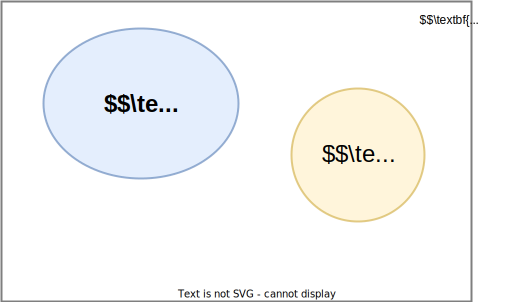
\includegraphics[scale=0.35]{figs/twoevents}
\par\end{center}

\end{frame}

\begin{frame}{\textbf{\textcolor{orange}{Betingade sannolikheter bäst i form av
träd}}}
\begin{center}
\includegraphics[scale=0.65]{figs/treecats}
\par\end{center}

\end{frame}

\begin{frame}{\textbf{\textcolor{orange}{Snitt- och marginella sannolikheter bäst
i tabell}}}
\begin{center}
\includegraphics[scale=0.65]{figs/pets_marginal_joint}
\par\end{center}

\end{frame}

\begin{frame}{\textbf{\textcolor{orange}{Bayes sats}}}
\begin{itemize}
\item \textbf{\textcolor{blue}{Allmänna multiplikationsregeln}}
\[
P(A\cap B)=P(B|A)P(A)=P(A|B)P(B)
\]
\item \textbf{\textcolor{blue}{Betingad sannolikhet}}
\[
P(B|A)=\frac{P(A\cap B)}{P(A)}
\]
\item \textbf{\textcolor{orange}{Bayes sats \emoji{smiling-face-with-heart-eyes}}}
\[
P(B|A)=\frac{P(A\vert B)P(B)}{P(A)}
\]
\item \textbf{\textcolor{blue}{Bayes vänder betingningar}}: beräkna $P(B\vert A)$
från \textrm{$P(A\vert B)$.} 
\end{itemize}
\end{frame}

\begin{frame}{\textbf{\textcolor{orange}{Känna igen handskrivna siffror}}}
\begin{itemize}
\item Förenkling: skilja på enbart 0:or och 1:or
\end{itemize}
\begin{center}
\includegraphics[scale=0.09]{figs/mnistZeroWithRedVoxel}\includegraphics[scale=0.09]{figs/mnistOneWithRedVoxel}
\par\end{center}
\begin{itemize}
\item {\small{}$A=$\{vit pixel i mitten\} och $B=$\{siffran är en nolla\}
\[
P(B\vert A)=\frac{P(A\vert B)P(B)}{P(A)}
\]
\[
P(B)=\frac{\text{antal bilder med nollor}}{\text{totalt antal bilder}}
\]
\[
P(A)=\frac{\text{antal bilder med vit pixel i mitten}}{\text{totalt antal bilder}}
\]
\[
P(A\vert B)=\frac{\text{antal bilder med nolla som också har vit pixel i mitten}}{\text{antal bilder med nollor}}
\]
}{\small\par}
\end{itemize}
\end{frame}

\begin{frame}{\textbf{\textcolor{orange}{Lagen om total sannolikhet}}}
\begin{itemize}
\item Sannolikheten för varje händelse $A$ kan delas upp som:
\[
P(A)={\normalcolor \textcolor{orange}{P(A\cap B)}}+\textcolor{blue}{P(A\cap B^{c})}
\]
\end{itemize}
\begin{center}
\includegraphics[scale=0.33]{figs/lawoftotalprob}
\par\end{center}
\begin{itemize}
\item Allmänna multiplikationsregeln: 
\[
\textcolor{orange}{P(A\cap B)=P(A\vert B)P(B)}\text{ och }\textcolor{blue}{P(A\cap B^{c})=P(A\vert B^{c})P(B^{c})}
\]
\item \textbf{\textcolor{blue}{Lagen om total sannolikhet}}
\[
P(A)=\textcolor{orange}{P(A\vert B)P(B)}+\textcolor{blue}{P(A\vert B^{c})P(B^{c})}
\]
\end{itemize}
\end{frame}

\begin{frame}{\textbf{\textcolor{orange}{Bayes sats - via lagen om total sannolikhet}}}
\begin{itemize}
\item \textbf{\textcolor{blue}{Lagen om total sannolikhet}}
\[
P(A)=P(A\vert B)P(B)+P(A\vert B^{c})P(B^{c})
\]
\item Bayes sats
\end{itemize}
\begin{center}
\[
P(B|A)=\frac{P(A\vert B)P(B)}{P(A)}
\]
\par\end{center}
\begin{itemize}
\item \textbf{\textcolor{blue}{Bayes sats }}med lagen om total sannolikhet
\[
P(B|A)=\frac{P(A\vert B)P(B)}{P(A\vert B)P(B)+P(A\vert B^{c})P(B^{c})}
\]
\end{itemize}
\end{frame}

\begin{frame}{\textbf{\textcolor{orange}{Fungerar hemtest för Covid?}}}
\begin{itemize}
\item \textbf{\textcolor{blue}{Bayes sats}}
\[
P(B|A)=\frac{P(A\vert B)P(B)}{P(A\vert B)P(B)+P(A\vert B^{c})P(B^{c})}
\]
\item Covid: A = \{pos\}. B = \{covid\}{\small{}
\[
P(\text{covid}\vert\text{pos})=\frac{P(\text{pos}\vert\text{covid})P(\text{covid})}{P(\text{pos}\vert\text{covid})P(\text{covid})+P(\text{pos}\vert\text{inte covid})P(\text{inte covid})}
\]
}{\small\par}
\item Notera: $P(\text{neg}\vert\text{inte covid})=1-P(\text{pos}\vert\text{inte covid})$.\medskip{}
\end{itemize}
\noindent{\fboxrule 1pt\fboxsep 5pt\fcolorbox{orange}{white}{\begin{minipage}[t]{1\columnwidth - 2\fboxsep - 2\fboxrule}%
\begin{itemize}
\item \textbf{\textcolor{blue}{Prevalens}}: $P(\text{covid})$ - andel med
covid i populationen.
\item \textbf{\textcolor{blue}{Sensitivitet}}: $P(\text{pos}\vert\text{covid})$
- hur \textbf{\textcolor{orange}{känsligt}} är testet för att upptäcka
covid?
\item \textbf{\textcolor{blue}{Specificitet}}: $P(\text{neg}\vert\text{inte covid})$
- är testet \textbf{\textcolor{orange}{specifikt}} för covid, eller
reagerar det även på annat?
\end{itemize}
%
\end{minipage}}}
\end{frame}

\begin{frame}{\textbf{\textcolor{orange}{Fungerar hemtest för covid?}}}
\begin{center}
\includegraphics[scale=0.25]{figs/covidtest_realtest}
\par\end{center}
\begin{itemize}
\item Sensitivitet: $P(\text{pos test}\vert\text{covid})=0.9677$
\item Specificitet: $P(\text{neg test}\vert\text{inte covid})=0.9920$
\end{itemize}
\begin{center}
\noindent{\fboxrule 1pt\fboxsep 1pt\fcolorbox{orange}{white}{\begin{minipage}[t]{1\columnwidth - 2\fboxsep - 2\fboxrule}%
\begin{center}
\href{https://statisticssu.github.io/SDA1/observable/bayestheorem.html}{\includegraphics[width=0.7\textwidth]{figs/bayessatswidget.png}}
\par\end{center}%
\end{minipage}}}
\par\end{center}
\begin{itemize}
\item {\footnotesize{}Notera dock att vanligtvis är $P(\text{covid}\vert\text{symptom})$
större än prevalensen $P(\text{covid})$. Man testar sig pga symptom.
Se slutet av denna }\textcolor{blue}{\footnotesize{}\uline{\href{https://observablehq.com/@mattiasvillani/bayes-theorem-for-events}{notebook}}}{\footnotesize{}.}{\footnotesize\par}
\end{itemize}
\end{frame}

\begin{frame}{\textbf{\textcolor{orange}{Lagen om total sannolikhet - allmän version}}}
\begin{center}
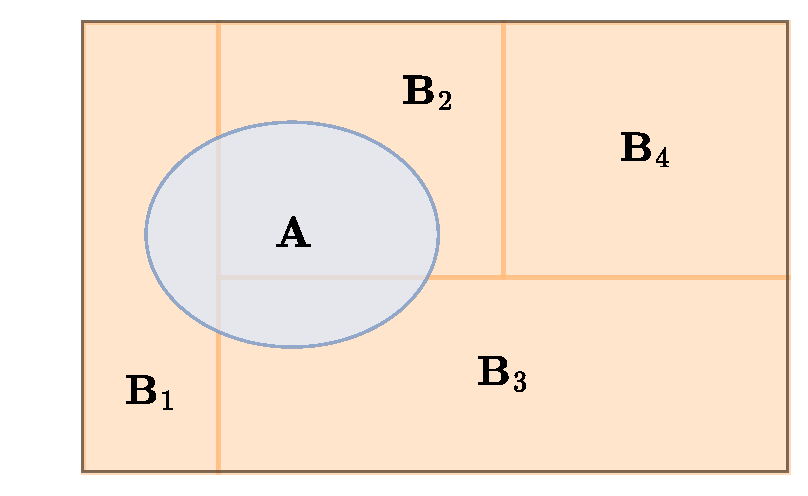
\includegraphics[scale=0.35]{figs/bayesgeneral}
\par\end{center}

\[
P(A)=\sum_{j=1}^{K}P(A|B_{j})p(B_{j})
\]

\end{frame}

\begin{frame}{\textbf{\textcolor{orange}{Bayes sats - allmän version}}}
\begin{center}
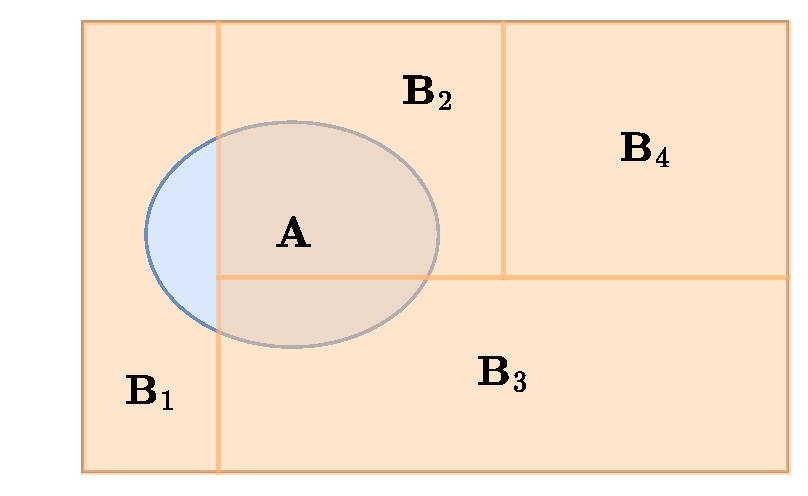
\includegraphics[scale=0.35]{figs/bayesgeneralwithintersect}
\par\end{center}

\[
P(B_{k}|A)=\frac{P(A|B_{k})P(B_{k})}{\sum_{j=1}^{K}P(A|B_{j})p(B_{j})}
\]

\begin{itemize}
\item Exempel: handskrivna siffor:\smallskip{}

\begin{itemize}
\item $B_{0}=$\{nolla\}, $B_{1}=$ \{etta\}, $B_{2}=$ \{tvåa\}, ... ,
$B_{9}=$ \{nia\}.\smallskip{}
\item $A=$\{vit pixel i mitten\}
\end{itemize}
\end{itemize}
\end{frame}

\begin{frame}{\textbf{\textcolor{orange}{Credits}}}

Dessa slides skapades för kursen statistik och dataanalys 1 av Mattias
Villani HT 2023, och har modifierats av Oscar Oelrich VT 2024, och
Oskar Gustafsson för VT 2025.
\end{frame}

\end{document}
